\documentclass[fleqn]{article}
\usepackage[spanish]{babel}
\usepackage{amsmath}
\usepackage{amsthm}
\usepackage{graphicx}
\usepackage[utf8]{inputenc}

%%%%%%%% MARGIN
\usepackage[left=1in, right=1in, top=0.8in, bottom=0.8in]{geometry}

%%%%%%%% NO PARAGRAPH INDENT
% https://tex.stackexchange.com/questions/27802/set-noindent-for-entire-file
\setlength\parindent{0pt}

%%%%%%%% SUB-FIGURE PACKAGE
\usepackage{subcaption}

\usepackage{pdfpages}

%%%%%%%% HYPERREF PACKAGE
\usepackage{hyperref}
\hypersetup{linkcolor=blue}
\hypersetup{citecolor=blue}
\hypersetup{urlcolor=blue}
\hypersetup{colorlinks=true}

%%%%%%%% MULTI-COLUMNS PACKAGE
\usepackage{multicol}

%%%%%%%% SETS DEFINITIONS
\usepackage{amssymb}
%%%% Important sets
\renewcommand{\O}{\mathbb{O}}
\newcommand{\N}{\mathbb{N}}
\newcommand{\Z}{{\mathbb{Z}}}
\newcommand{\Q}{{\mathbb{Q}}}
\newcommand{\RR}{{\mathbb{R}}}

%%%% Statistics
\newcommand{\E}[1]{\mathbb{E}\left[#1 \right]}
\newcommand{\V}[1]{\mathbb{V}\left[#1 \right]}
\newcommand{\cov}[1]{\mathrm{Cov}\left[#1 \right]}

%%% Misc Math
% Spaces after/before left/right
\let\originalleft\left
\let\originalright\right
\renewcommand{\left}{\mathopen{}\mathclose\bgroup\originalleft}
\renewcommand{\right}{\aftergroup\egroup\originalright}

% Norm and abs
\newcommand{\norm}[1]{\left\lVert#1\right\rVert}
\newcommand{\abs}[1]{\left\lvert#1\right\rvert}

%%%% Superscript to the left
% https://latex.org/forum/viewtopic.php?t=455
\usepackage{tensor}
\newcommand{\app}[3]{\tensor*[^{#1}]{\left(#2, #3\right)}{}}


%%%%%%%% SPLIT EQUATIONS
% https://tex.stackexchange.com/questions/51682/is-it-possible-to-pagebreak-aligned-equations
\allowdisplaybreaks

%%%%%%%% CODE RENDERING
% Compile with flag -shell-escape
\usepackage{minted}

%%%%%%%% EXAM PACKAGE
\usepackage{mathexam}

%%%%%%%% CHANGE MARGINS ITEMIZE
\usepackage{enumitem}

%%%%%%%% START DOCUMENT

\ExamClass{CM0091 - Inteligencia Artificial}
\ExamName{Examen ANN}
\ExamHead{\today}

\let\ds\displaystyle

\begin{document}
 \vspace{0.3cm}
   % Information of the student
   \begin{itemize}[leftmargin=6.25cm, labelsep=0.5cm]

     \item[\textit{Nombre}] \scalebox{1.2}{David Plazas Escudero} % Name
     \item[\textit{Código}] 201710005101 % Code

   \end{itemize}
\vspace{0.3cm}

% Each of the items to solve
\begin{enumerate}
    \item \textit{¿Cuál es la dinámica más fácil y la más difícil de aprender?}
    De la Figura \ref{fig:outs} se puede observar que la dinámica más fácil de aprender es el crecimiento y el punto de quiebre, pues en todos los conjuntos, la red saca resultados similares a la dinámica real. No obstante, hay tres comportamientos que no logra reproducir correctamente: la altura del pico, la condición inicial y la pendiente de caída. Por lo tanto, estas son las dinámicas más difíciles de aprender.
    
    Es importante resaltar que el número de épocas (50) todavía es pequeño para que la red pueda generalizar correctamente el comportamiento, pues en la Figura \ref{fig:grads} se observa que todavía no han convergido completamente a 0.
    \begin{figure}[H]
    \centering
    \begin{subfigure}[b]{0.45\textwidth}
        \centering
        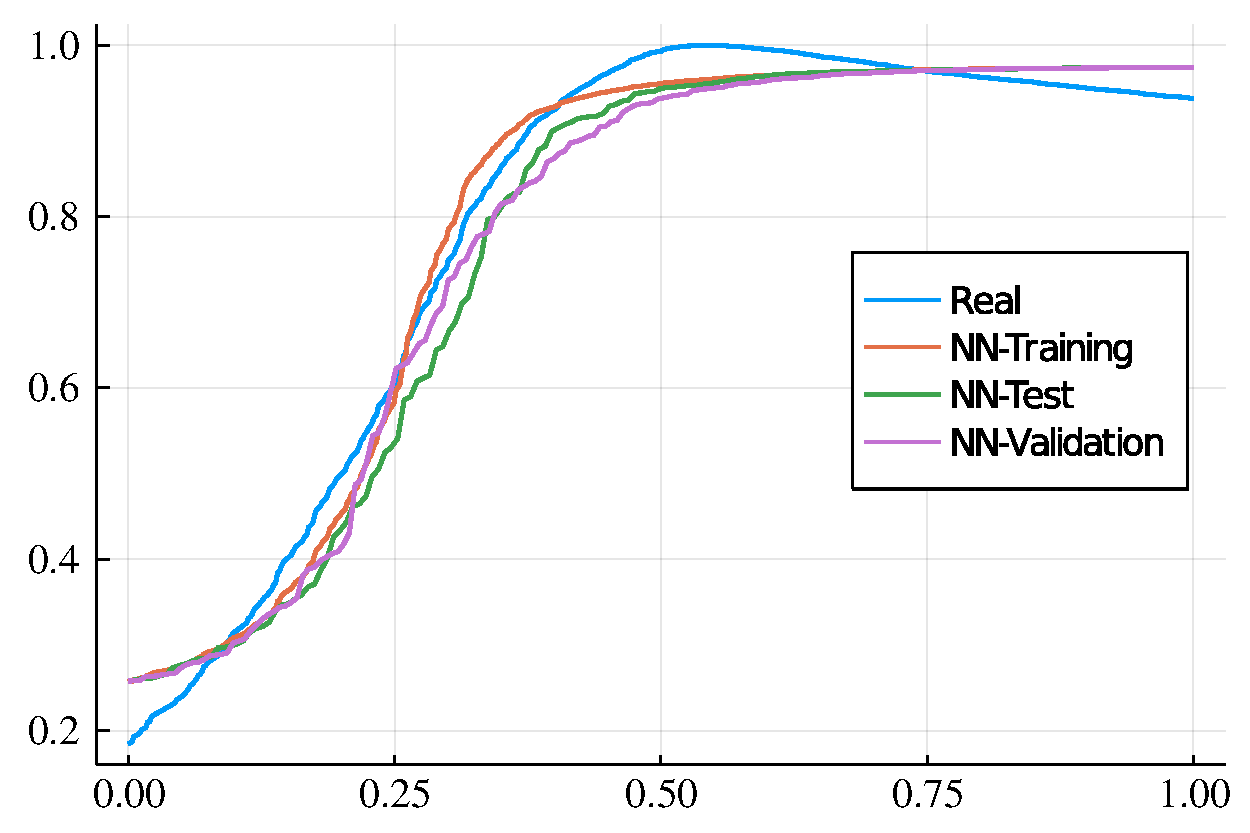
\includegraphics[width=\textwidth]{2/output.pdf}
        \caption{$\eta=0.2$.}
    \end{subfigure}
    \begin{subfigure}[b]{0.45\textwidth}  
        \centering 
        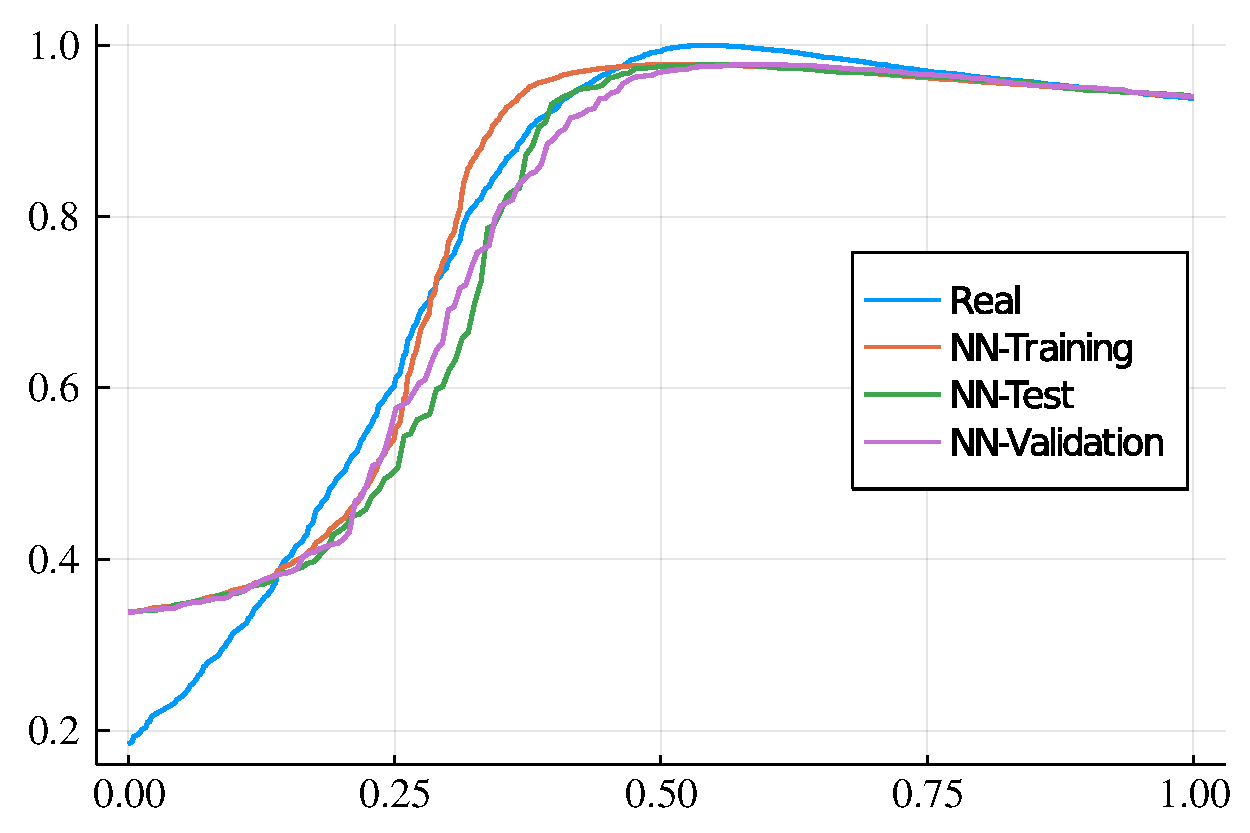
\includegraphics[width=\textwidth]{9/output.pdf}
        \caption{$\eta=0.9$.}
    \end{subfigure}
    \caption{Salida real vs. red neuronal para los diferentes conjuntos para dos $\eta$.}
    \label{fig:outs}
    \end{figure}
    
    \begin{figure}[H]
    \centering
    \begin{subfigure}[b]{0.45\textwidth}
        \centering
        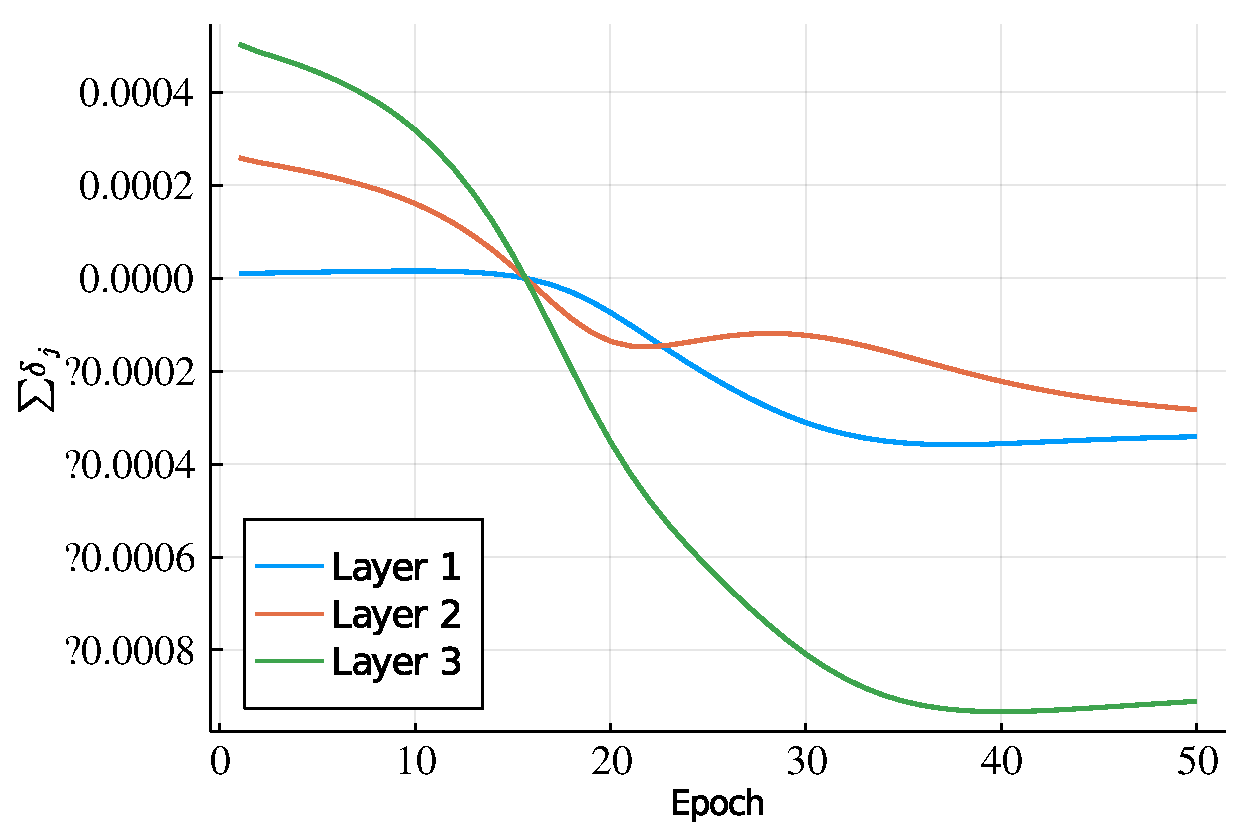
\includegraphics[width=\textwidth]{2/grads.pdf}
        \caption{$\eta=0.2$.}
    \end{subfigure}
    \begin{subfigure}[b]{0.45\textwidth}  
        \centering 
        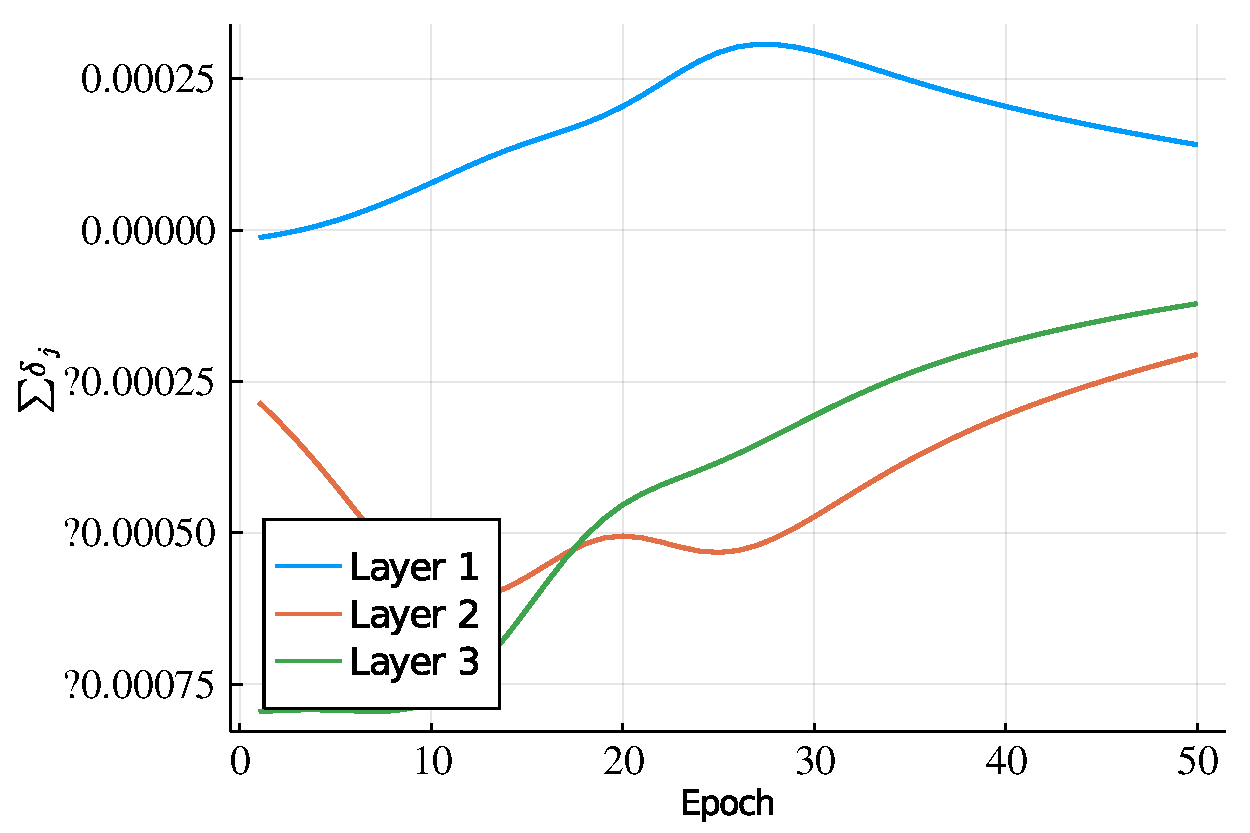
\includegraphics[width=\textwidth]{9/grads.pdf}
        \caption{$\eta=0.9$.}
    \end{subfigure}
    \caption{Suma de gradientes en redes neuronales por capa.}
    \label{fig:grads}
    \end{figure}
    
    \begin{figure}[H]
    \centering
    \begin{subfigure}[b]{0.45\textwidth}
        \centering
        \includegraphics[width=\textwidth]{2/Eav.pdf}
        \caption{$\eta=0.2$.}
        \label{fig:2}
    \end{subfigure}
    \begin{subfigure}[b]{0.45\textwidth}  
        \centering 
        \includegraphics[width=\textwidth]{9/Eav.pdf}
        \caption{$\eta=0.9$.}
        \label{fig:9}
    \end{subfigure}
    \caption{Energía del error promedio.}
    \label{fig:eav}
    \end{figure}
    
    

\end{enumerate}
\end{document}
